\documentclass[tikz,border=2pt]{standalone}
\usepackage{lmodern}
\usepackage{pgfplots}
\pgfplotsset{compat=1.18,every axis/.append style={
 font=\fontsize{9}{11}\selectfont,tick label style={font=\fontsize{9}{11}\selectfont},
 label style={font=\fontsize{9}{11}\selectfont},title style={font=\fontsize{9}{11}\selectfont},
 axis line style={black!50,line width=.4pt},tick style={black!50},
 axis lines*=left,clip=false,legend style={draw=none,font=\fontsize{9}{11}\selectfont},
 scaled ticks=false}}
\definecolor{accent}{HTML}{365F7D}
\begin{document}
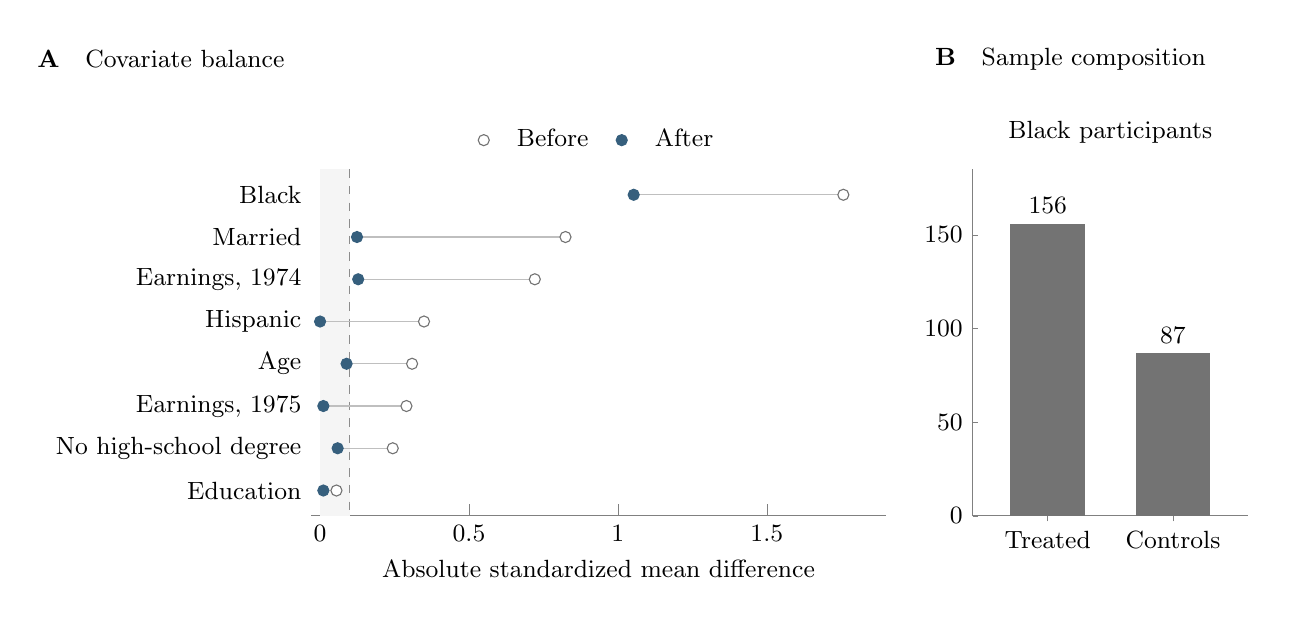
\begin{tikzpicture}[font=\fontsize{9}{11}\selectfont]
\path[use as bounding box] (0,0) rectangle (16,7.4);
\node[anchor=west] at (0,7.0) {\textbf{A}\quad Covariate balance};
\node[anchor=west] at (11.4,7.0) {\textbf{B}\quad Sample composition};
\begin{axis}[at={(3.6cm,1.2cm)},anchor=south west,width=7.3cm,height=4.4cm,scale only axis,
 xmin=-.03,xmax=1.9,ymin=-.6,ymax=7.6,y dir=reverse,ytick={0,1,2,3,4,5,6,7},
 yticklabels={{Black},{Married},{Earnings, 1974},{Hispanic},{Age},{Earnings, 1975},{No high-school degree},{Education}},
 xtick={0,.5,1,1.5},xlabel={Absolute standardized mean difference},
 y axis line style={draw=none},ytick style={draw=none},legend columns=2,
 legend style={at={(.5,1.02)},anchor=south,column sep=8pt}]
\fill[black!4] (axis cs:0,-.6) rectangle (axis cs:.1,7.6);
\draw[dashed,black!45] (axis cs:.1,-.6) -- (axis cs:.1,7.6);
\draw[black!25] (axis cs:1.757,0) -- (axis cs:1.053,0);
\draw[black!25] (axis cs:0.824,1) -- (axis cs:0.124,1);
\draw[black!25] (axis cs:0.721,2) -- (axis cs:0.128,2);
\draw[black!25] (axis cs:0.349,3) -- (axis cs:0,3);
\draw[black!25] (axis cs:0.309,4) -- (axis cs:0.089,4);
\draw[black!25] (axis cs:0.29,5) -- (axis cs:0.011,5);
\draw[black!25] (axis cs:0.244,6) -- (axis cs:0.059,6);
\draw[black!25] (axis cs:0.055,7) -- (axis cs:0.011,7);
\addplot[only marks,mark=*,mark size=2pt,black!55,mark options={fill=white}] coordinates {(1.757,0) (0.824,1) (0.721,2) (0.349,3) (0.309,4) (0.29,5) (0.244,6) (0.055,7)};
\addlegendentry{Before}
\addplot[only marks,mark=*,mark size=2pt,accent] coordinates {(1.053,0) (0.124,1) (0.128,2) (0,3) (0.089,4) (0.011,5) (0.059,6) (0.011,7)};
\addlegendentry{After}
\end{axis}
\begin{axis}[at={(12cm,1.2cm)},anchor=south west,width=3.5cm,height=4.4cm,scale only axis,
 ybar,bar width=27pt,bar shift=0pt,ymin=0,ymax=185,xmin=-.6,xmax=1.6,
 xtick={0,1},xticklabels={Treated,Controls},ytick={0,50,100,150},
 title={Black participants},tickwidth=2pt]
\addplot[fill=black!55,draw=none] coordinates {(0,156)};
\addplot[fill=black!55,draw=none] coordinates {(1,87)};
\node[anchor=south] at (axis cs:0,156) {156};
\node[anchor=south] at (axis cs:1,87) {87};
\end{axis}
\end{tikzpicture}
\end{document}
